\documentclass[dvipdfmx,a4paper]{jreport} % dvipdfmxオプションを追加
\usepackage{amsmath,amssymb}
\usepackage{graphicx}
\usepackage{url} % ウェブサイトのURLをきれいに表示するため
\usepackage{multicol} % 必要であれば多段組用
\usepackage{caption} % 図表のキャプション設定
\usepackage{subcaption} % subfigure環境用
\usepackage{float} % [H]オプションを使うため

% 日本語設定
\usepackage[utf8]{inputenc}
\usepackage[T1]{fontenc}
\usepackage{otf}
\usepackage[ipaex]{pxchfon} % IPAexフォントを使用 (pxgothicの代わりに推奨)

\usepackage{geometry}
\geometry{a4paper,
  top=30mm,
  bottom=30mm,
  left=25mm,
  right=25mm
}

% タイトルページの作成
\makeatletter
\def\titlepage{%
  \thispagestyle{empty}%
  \begin{center}%
    \vspace*{\fill}%
    {\huge \bfseries 船舶の横揺れ運動に関する実験レポート \\}%
    \vspace{2cm}%
    {\large 実施日時:6月24日\\}%
    \vspace{1cm}%
    {\large 2班 \\}%
    \vspace{1cm}%
    {\large 学籍番号:08C23031\\}%
    \vspace{1cm}%
    {\large 氏名:古賀 光一朗 \\}%
    \vspace*{\fill}%
  \end{center}%
}
\makeatother

\begin{document}

\titlepage

---

\chapter{目的}
本実験は、船舶の復原性試験を実施し、船舶や浮体構造物の模型実験に必要な基本的なバラスティング作業および波浪中での復原性試験法を習得することを目的とする。また、傾斜試験や自由横揺れ試験で得られたデータの解析を通じて浮体の横揺れに関する理解を深め、浮体静力学および船舶復原論で学習した内容を実験を通じて実際の現象として理解することを目的とする。

---

\chapter{方法}
\section{実験場所および装置}
本実験は、大阪大学船舶海洋試験水槽(S3棟)にて実施した。水槽の主な設備仕様は以下の通りである。

\begin{itemize}
    \item \textbf{水槽:} 長さ 100m, 幅 7.8m, 水深 4.35m
    \item \textbf{レール:} 50kg/mレール, 頭部上面及び側面機械加工, 継目板溶接
    \item \textbf{曳引車:} 長さ 7.4m, 幅 7.8m, ホイール・ベース 6.4m, 鋼製ボックス・ガーダー構造, 総重量 20t, 駆動モーター ACサーボ7.5KW 4台, 走行速度 0.01~3.5 m/s, 速度制御ディジタル方式によるトルクバランス制御, 速度設定精度 $\pm 0.01\%$以下, 速度安定度 0.05\% r.m.s.
    \item \textbf{造波機:} プランジャー式, 駆動モーター 11KW 2台, 最大波高 500mm, 波長 0.5~15m, 一方向不規則波発生可能
    \item \textbf{消波装置:} 水槽端に固定式すのこビーチ・ヘチマロン, 側壁に可動式ビーチ
    \item \textbf{濾過装置:} 循環式濾過装置 処理能力 40t/h
\end{itemize}

\section{使用模型船}
本実験では、1/70縮尺のSR108コンテナ模型船を使用した。この船の主要目を表\ref{tab:principal_particulars}に示す。

\begin{table}[htbp]
    \caption{主要目}
    \label{tab:principal_particulars}
    \centering
    \begin{tabular}{|l|l|}
        \hline
        \textbf{供試船} & \textbf{値} \\
        \hline
        垂線間長 : $L_{pp}$ & 2.50 m \\
        型幅 : $B$ & 0.363 m \\
        深さ : $D$ & 0.233 m \\
        喫水(F.P., midship, A.P.) & 0.136 m \\
        方形係数 : $C_b$ & 0.557 \\
        標準メタセンター高さ : $GM$ & 0.020 m \\
        排水体積: $V$ & 0.0688 m$^3$ \\
        \hline
    \end{tabular}
\end{table}
また正面線図は、以下である。
\begin{figure}[H] % floatパッケージのHオプションを使用
    \centering
    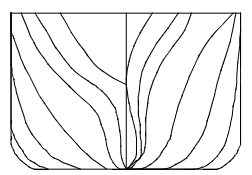
\includegraphics[width=0.45\textwidth]{summer/ship-experiment/long-pool/buttock-lines.png} % 実際の図のファイル名に変更 (実験要領の図6)
     \caption{正面線図}
     \label{fig:Buttock lines}
\end{figure}

\section{実験手順}
浮体の模型実験における基礎的な準備作業・試験項目であるバラスティング・傾斜試験、自由横揺れ試験を実施した。さらに、縦波中を曳航してパラメトリック横揺れに関する復原性試験を実施した。

\subsection{バラスティング}
バラスティング作業では、まず模型船単独の重量を台はかりで計測し、所定の排水体積相当の重量(排水量)から差し引くことで必要となるバラスト総重量を確認した。排水量を求める際には、事前に計測された水槽の水の密度 $0.9997 \text{ g/cm}^3$ を用いた。次に、模型船を水に浮かべた状態でバラストウェイトを安定な位置に配置し、排水量および初期トリムを所定の値に合わせた。船体中央、船首部、船尾部の両舷側から見て、模型船の喫水線と静水面が一致すれば、排水量と初期トリムが横傾斜無しの状態で満たされたと判断した。

 \begin{figure}[H] % floatパッケージのHオプションを使用
     \centering
     \begin{subfigure}[b]{0.45\textwidth}
         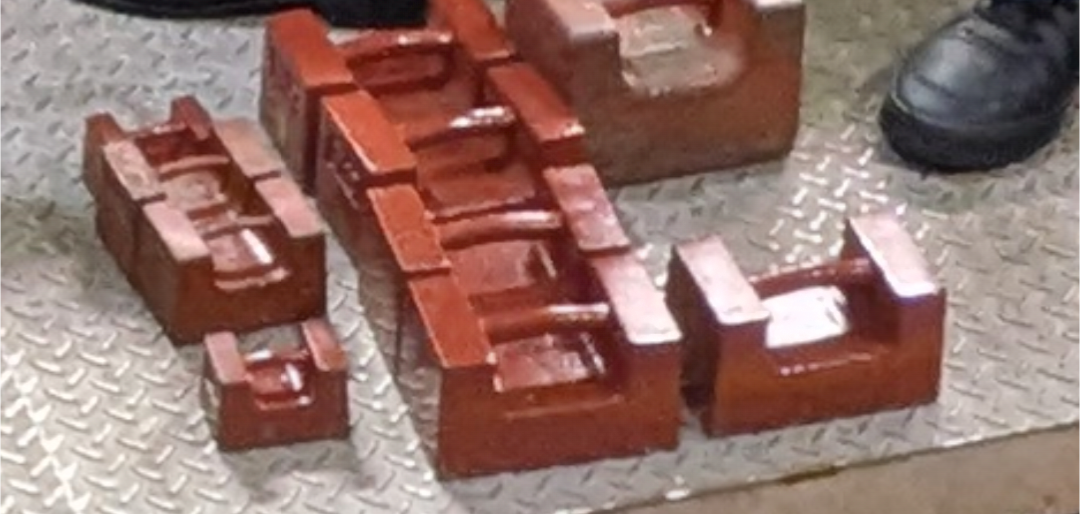
\includegraphics[width=\textwidth]{summer/ship-experiment/long-pool/ballast_weight.png} % 実際の図のファイル名に変更 (実験要領の図4)
         \caption{バラストウェイト}
         \label{fig:ballast_weight}
     \end{subfigure}
     \hfill
     \begin{subfigure}[b]{0.45\textwidth}
         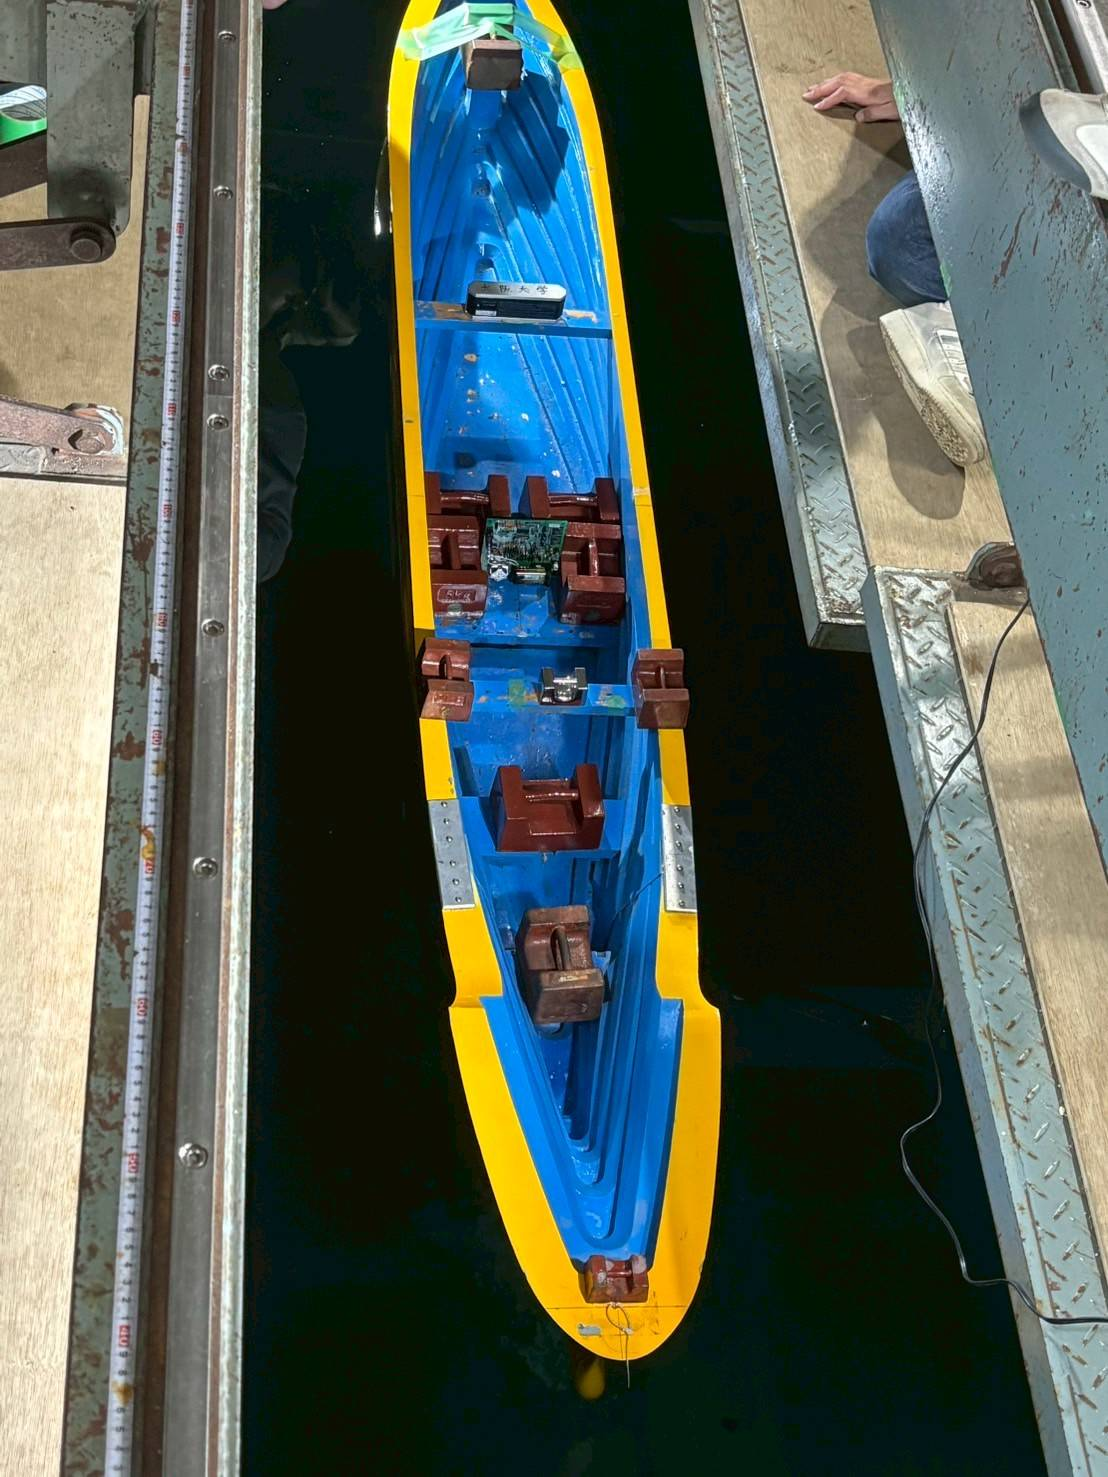
\includegraphics[width=\textwidth]{summer/ship-experiment/long-pool/ballast_arrangement.png} % 実際の図のファイル名に変更 (実験要領の図5)
         \caption{バラストウェイトの配置}
         \label{fig:ballast_arrangement}
     \end{subfigure}
     \caption{バラスティング関連図}
 \end{figure}


\subsection{傾斜試験}
傾斜試験は、船舶の復原性能を表す最も基本的な指標であるメタセンター高さ($GM$)を計測するために実施した。まず、模型船を水に浮かべた状態で船体長手方向重心位置付近にデジタル傾斜計を設置し、傾斜角を計測した。次に、船内に配置されたバラストウェイトのうち適度な重さのウェイトを前後方向位置を保持したまま片舷に移動させ、その時の傾斜角を計測した。その後、このバラストウェイトを反対舷に移動させ、この移動に伴う模型船の横傾斜角の変化量を計測し、重心まわりのモーメントの釣り合いを表す以下の式から$GM$を求めた。

$$ GM = \frac{w l}{W \tan \theta} \quad [\text{m}] \quad \text{} $$
$w$: 移動させたバラストウェイトの重量 [$kg$]\\
$l$: バラストウェイトの移動量 [$m$]\\
$W$: 排水量 [$kg$]\\
$\theta$: バラストウェイトの移動による模型船のヨコ傾斜角の変化量[$deg$]\\
\\
$GM$の目標値は表\ref{tab:principal_particulars}に示す値とし、バラストウェイトの上下移動と傾斜試験を2回繰り返した。バラストウェイトの前後移動を行う場合は、初期トリムと横傾斜を再確認した。この際、デジタル傾斜計搭載による重心高さの変化は微小として無視した。

 \begin{figure}[H] % floatパッケージのHオプションを使用
     \centering
     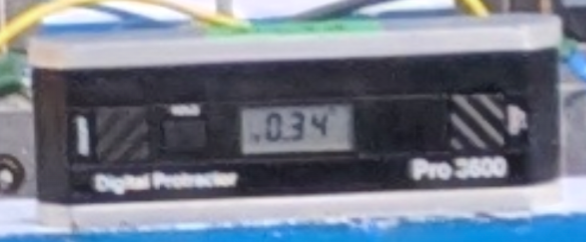
\includegraphics[width=0.45\textwidth]{summer/ship-experiment/long-pool/digital_inclinometer.png} % 実際の図のファイル名に変更 (実験要領の図6)
     \caption{デジタル傾斜計}
     \label{fig:digital_inclinometer}
 \end{figure}


\subsection{自由横揺れ試験}
船体横揺れ運動を計測するため、模型船に振動式ジャイロスコープを取り付けた。計測精度の観点から、ジャイロスコープは船体重心位置に近付けて設置することが望ましい。水槽側壁からの波の反射影響を避けるため、曳航台車を用いて模型船を側面消波板のある40m付近まで移動させた。水に浮かべた模型船を片側に横傾斜を与えて静止させ、ある瞬間にその傾斜拘束を解除し、その後に発生する横揺れの減衰運動を、ジャイロスコープを用いて横揺れがほぼ減衰するまでの時刻暦を計測した。この際、できるだけ大きな初期傾斜を与えるよう努めたが、模型船内に水が流入しないように注意した。また、大きな漂流や回頭運動が発生した場合はやり直した。自由横揺れ試験は前進速度が無い場合とした。


\subsection{パラメトリック横揺れ試験}
波長船長比 $\lambda/L_{pp}=1$、波岨度 $H/\lambda=0.01$ の規則縦波中で、ジャイロスコープを用いて船体横揺れ運動を計測した。曳航台車を用いて模型船を曳航することで前進速度を変更し、パラメトリック横揺れの発生を試みた。$GM$を変更した場合は、実験後に再度傾斜試験を実施した。

パラメトリック横揺れは、以下の不等式が満たされる時に発生するとされる。
$$ \left(\frac{GM_{amp}}{GM}\right)^2 > 4 \left[1 - \left(\frac{\omega}{\omega_\phi}\right)^2\right]^2 + 16 \left(\frac{\omega}{\omega_\phi}\right)^2 \left(\frac{\alpha}{\omega_\phi}\right)^2 \quad \text{} $$
ここで、$GM$は計測値、波長船長比 $\lambda/L_{pp}=1$、波岨度 $H/\lambda=0.01$ の規則縦波中での復原力変動振幅 $GM_{amp}$ は、$0.00157 \text{ [m]}$とする。$\omega$はパラメトリック横揺れの角周波数であり、出会い波周波数 $\omega_e$ の半分、すなわち $\omega=\omega_e/2$ で表される。出会い波角周波数 $\omega_e$ は、入射波の波長 $\lambda$ とフルード数 $Fn$、船長 $L_{pp}$ を用いて、以下で定義される。
$$ \omega_e = \sqrt{\frac{2\pi g}{\lambda}} \left(1 - \sqrt{\frac{2\pi}{\lambda}L_{pp}} Fn\right) \quad \text{} $$
フルード数 $Fn$ は船速 $U$ [m/s](追波を正、向波を負で定義)の無次元値であり、重力加速度 $g=9.81 \text{ [m/s}^2\text{]}$ を用いて以下で定義される。
$$ Fn = \frac{U}{\sqrt{L_{pp} g}} \quad \text{} $$
$\omega_\phi$ および $\alpha$ は横揺れ固有周波数および線形の減衰係数であり、自由横揺れ試験を解析することで求める。$\alpha$ については、後述の減滅曲線の1次の係数を $a$、横揺れ固有周期を $T_\phi$ とすると、以下で求められる。
$$ \alpha = \frac{2a}{T_\phi} \quad \text{} $$
実験の際は、概略 $a=0.017$ とし、$T_\phi$ は自由横揺れ試験の際にストップウォッチで計測し、パラメトリック横揺れが発生する船速を推定した。

\subsection{準拠標準}
本実験は、以下の標準に準拠して実施した。
\begin{itemize}
    \item IMO: INTERIM GUIDELINES FOR ALTERNATIVE ASSESSMENT OF THE WEATHER CRITERION, MSC.1/Circ. 1200, 2006.
    \item IMO: INTERNATIONAL CODE ON INTACT STABILITY, 2008, Annex 1 Detailed guidance for the conduct of an inclining test, 2009.
\end{itemize}

---

\chapter{結果}
\section{重量計測結果}
模型船の船殻重量は$27.7kg$であった。

\section{GM調整結果}
傾斜試験の結果を以下の表にまとめる。


今回は、$500g$の錘を用いて
はじめの傾斜試験では$l=0.05(m)$とし、
実験後の傾斜試験では$l=0.03(m)$とした。
\begin{table}[htbp]
    \caption{GM}
    \label{table:gm}
    \centering
    \begin{tabular}{|l|l|}
        \hline
        \textbf{データラベル} & \textbf{GM値$(m)$} \\
        \hline
        実験前(傾斜試験)&0.0286\\
        自由横揺れの周期から推定&0.00883\\
        おもりの移動距離から推定&0.0067\\
        実験後(傾斜試験)&0.00625\\
        \hline
    \end{tabular}
\end{table}


\section{自由横揺れ試験}
自由横揺れ試験の結果、ジャイロスコープから得られたデータを台形積分することにより図\ref{fig:yokoyure}を得る。
 \begin{figure}[H] % floatパッケージのHオプションを使用
     \centering
     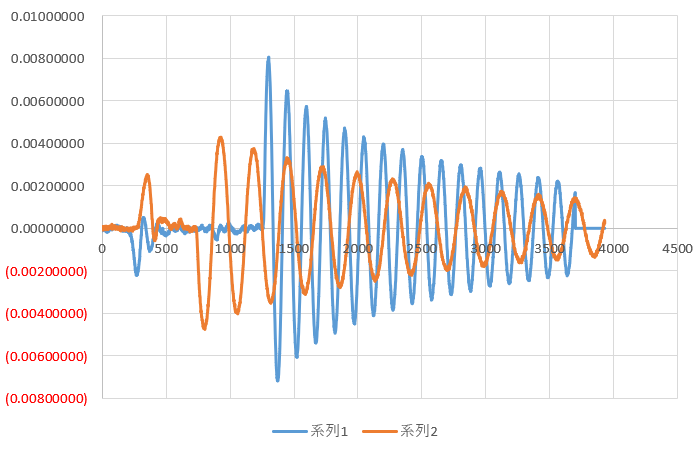
\includegraphics[width=0.8\textwidth]{summer/ship-experiment/long-pool/yokoyure.png} % 図のファイル名を適切に変更してください (実験要領の図2に相当)
     \caption{自由横揺れ試験での船体の傾きのふるまい}
     \label{fig:yokoyure}
 \end{figure}

\section{パラメトリック横揺れ試験}
パラメトリック横揺れ試験の詳細結果については添付のExcelシートを参照されたい。

---

\chapter{考察}
本章では、実験結果に基づいて、課題として与えられた内容について詳細に考察する。

\section{台はかりの使用方法とアナログはかりの利点}
\subsection{台はかりの使用方法}
\begin{enumerate}
  \item 水平な床に台はかりを置く
  \item 台はかりの目盛りのついた棒に刺さっている錘を根元に移動しておく
  \item 台はかりの上に計測する船体模型を置く
  \begin{enumerate}
      \item このとき、船体の重心をできるだけ真ん中に置くようにする
  \end{enumerate}
  \item その船型データに基づき、船殻重量より少し小さい値に相当する錘を台はかりの先端にある皿にのせる
  \item 台はかりの目盛りのついた棒に刺さっている錘をずらして、先端が水平につりあう点を探す
  \begin{enumerate}
      \item この釣り合う点と皿に乗っている錘の値を足し合わせることにより船殻重量が得られる。
  \end{enumerate}
\end{enumerate}

\subsection{アナログはかりのメリット}
考えられるメリットを以下に列挙する。
\begin{itemize}
    \item 電気回路を用いていないので電源が不要
    \item 電気回路を用いていないので金属粉などのごみにも強い
    \item センサーなどの繊細な部品がないため機械剛性を高めることができる
    \begin{itemize}
        \item これにより大重量物に対しても測定することができる
    \end{itemize}
    \item 半田の劣化等と無縁なので寿命が長い
    \item メンテナンスが容易
\end{itemize}


\section{横揺れ角計測機器の比較とジャイロスコープの使用理由}
\subsection{傾斜計とジャイロスコープの特徴}
自由横揺れ試験では、横揺れ角を傾斜計ではなくジャイロスコープで計測した。それぞれの計測機器の特徴を以下にまとめる。
\begin{itemize}
    \item \textbf{傾斜計:} 重力方向に対する傾きを直接計測する機器である。静的な傾斜や、非常にゆっくりとした傾斜の計測に適している。しかし、動的な運動、特に短周期の横揺れ運動に対しては、慣性力の影響を受けやすく、正確な追従が難しい場合がある。
    \item \textbf{ジャイロスコープ:} 角速度を検出する機器であり、これを時間で積分することで角度を算出する。振動式ジャイロは、内部で電磁気作用により共振振動するばね系に働くコリオリの力から系に作用する加速度を検出する。すなわち、角速度に比例する電圧を一定の時間間隔で出力する。動的な運動、特に横揺れのような比較的速い角運動の計測に優れている。ただし、角速度の計測誤差があると、時間積分により角度にドリフト(時間とともに誤差が累積する現象)が生じるという特徴がある。
\end{itemize}

\subsection{ジャイロスコープを用いた理由}
自由横揺れ試験において、傾斜計ではなくジャイロスコープを用いた理由は、横揺れ運動が時間とともに連続的に変化する動的な現象であり、ジャイロスコープの方がより高精度かつリアルタイムでこの動的な角運動を捉えるのに適しているためであると考えられる。傾斜計では、特に揺れが大きい場合や周期が短い場合に、慣性による誤差が大きくなり、正確な減衰曲線を計測することが困難となる可能性がある。ジャイロスコープはドリフト誤差の問題があるものの、適切なドリフト修正を行うことで、動的な横揺れ角の時系列データを正確に取得できる。

\subsubsection*{参考情報}
\begin{itemize}
    \item DifiKey Tech Forum , 閲覧日:2025/07/08
    
    \url{https://forum.digikey.com/t/topic/48459}
    
    \item Panasonic慣性センサの基礎知識~ジャイロセンサ、加速度センサ~, 閲覧日:2025/07/08

\url{https://industrial.panasonic.com/jp/ds/ss/technical/b14},

\end{itemize}

\section{GM調整過程の報告}

\subsection{初期状態での$GM$計測}
図\ref{table:gm}に記したように、初めのバラスト調整時には
$$GM=0.0286$$
であった。
これは、全ての錘を船底に配置したところ、GMが大きすぎたのである程度の錘を上に上げて重心が上がるように調整した結果である。

\subsection{パラメトリック横揺れ試験(1回目)をうけての再調整}
はじめの$GM$ではパラメトリック横揺れが起こらなかったので$GM$が大きすぎると考え、さらに錘を上げて重心を上げた。今度は自由横揺れ試験時の周期から$GM$を推定した。
自由横揺れ試験の結果$T_\phi$は$1.39$から$2.5$に変化し、これにより、$\omega_\phi$も$4.52$から$2.51$に変化した。
\begin{equation}
    GM_{new}=GM_{old}\times\frac{\omega_{new}^2}{\omega_{old}^2}
\end{equation}
であり、これにより
$$GM=0.00883$$
とわかった。

\subsection{パラメトリック横揺れ試験(2回目)をうけての再調整}
周期から推定した$GM$ではパラメトリック横揺れが起こらなかったので、推定の方法を見直し、重心移動から概算してみることにした。
その結果は
$$GM=0.0067$$
となった。

\subsection{最後に傾斜試験で確認}
重心移動から推定した$GM$の値でパラメトリック横揺れが実現したが、長水槽の曳引車の上で錘の移動を行ったため、傾斜試験ができておらず、正確な$GM$ではなく、推定した$GM$であったので、着岸した後に再度傾斜試験を行った。
その結果
$$GM=0.00625$$
となり、推定と大差ない結果が得られた。

\section{減衰曲線と減滅曲線}
\subsection{減衰曲線}
時系列データから作成した横揺れ減衰曲線を図\ref{fig:damping_curve_processed}に示す。この減衰曲線は、模型船をある角度だけ横傾斜させてから放すと、横揺れ角が横揺れ減衰力によるエネルギー散逸のために、一揺毎に減少していく様子を示している(実験要領の図2に相当)。

 \begin{figure}[H] % floatパッケージのHオプションを使用
     \centering
     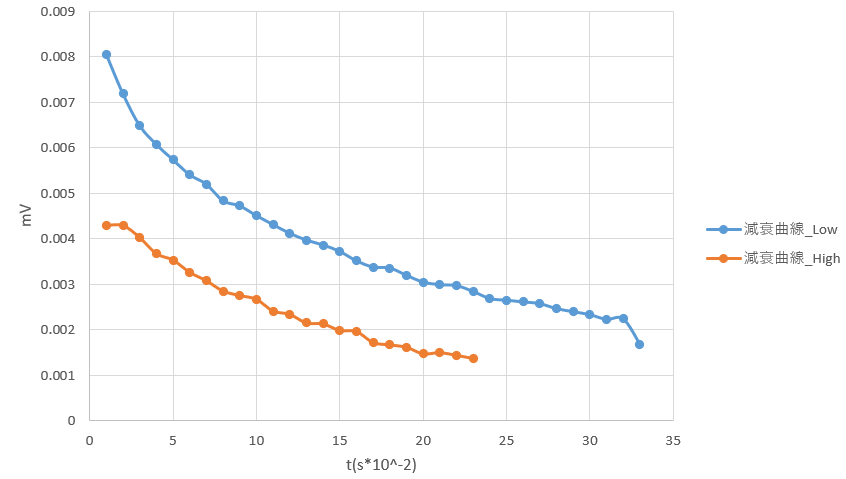
\includegraphics[width=0.8\textwidth]{summer/ship-experiment/long-pool/damping_curve_processed.png} % 図のファイル名を適切に変更してください (実験要領の図2に相当)
     \caption{横揺れ減衰曲線(実験要領の図2に相当)}
     \label{fig:damping_curve_processed}
 \end{figure}

\subsection{減滅曲線}
横揺れ減衰曲線から導出した減滅曲線を図\ref{fig:extinction_curve_01}と\ref{fig:extinction_curve_02}に示す。減滅曲線は、減衰曲線の相隣る二つの片振幅を $\phi_n$, $\phi_{n+1}$ とし、その差を $\Delta\phi = \phi_n - \phi_{n+1}$ とおく。また平均値を $\phi'_n = (\phi_n + \phi_{n+1})/2$ として、横軸に $\phi'_n$、縦軸に $\Delta\phi$ をとったグラフである(実験要領の図3に相当)。このグラフには2次の近似曲線と、その近似曲線を表す数式を示す。

 \begin{figure}[H] % floatパッケージのHオプションを使用
     \centering
     \begin{subfigure}[b]{0.45\textwidth}
         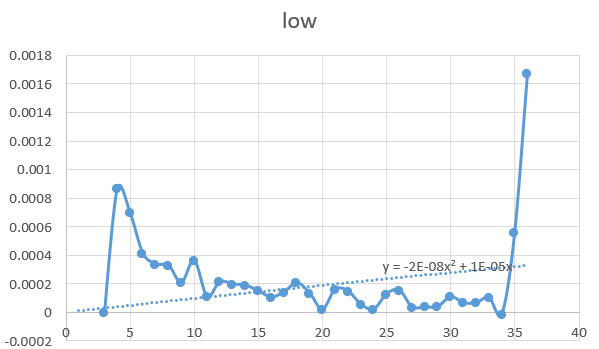
\includegraphics[width=\textwidth]{summer/ship-experiment/long-pool/extinction_curve_01.png} % 実際の図のファイル名に変更 (実験要領の図4)
         \caption{減滅曲線1回目}
         \label{fig:extinction_curve_01}
     \end{subfigure}
     \hfill
     \begin{subfigure}[b]{0.45\textwidth}
         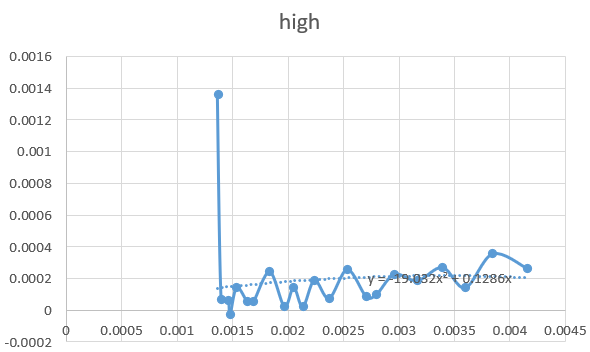
\includegraphics[width=\textwidth]{summer/ship-experiment/long-pool/extinction_curve_02.png} % 実際の図のファイル名に変更 (実験要領の図5)
         \caption{減滅曲線2回目}
         \label{fig:extinction_curve_02}
     \end{subfigure}
     \label{extinction_curve}
     \caption{減滅曲線}
 \end{figure}


\section{パラメトリック横揺れの推定と実験結果の比較考察}
5)で求めた減滅曲線の1次の係数 $B$ を$a$、横揺れ固有周期を $T_\phi$ とした場合の線形の減衰係数 $\alpha$ を $\alpha = 2a/T_\phi$ で求めた。この $\alpha$ および実験で計測した$GM$、そして$GM_{amp}=0.00157 \text{ [m]}$を用いて、パラメトリック横揺れが発生する条件式
\begin{equation}
   \left(\frac{GM_{amp}}{GM}\right)^2 > 4 \left[1 - \left(\frac{\omega}{\omega_\phi}\right)^2\right]^2 + 16 \left(\frac{\omega}{\omega_\phi}\right)^2 \left(\frac{\alpha}{\omega_\phi}\right)^2 
\end{equation}
を満たす船速 $U$ を推定した。
\vspace{5mm}


まず、初めの実験に注目してみる


初めの$GM$ではどの船速でも起こらないという計算結果であり、実際にも起こらなかった。これは$GM$が大きすぎた事に起因すると考えられる。

\vspace{5mm}
次に、錘を上げて周期から$GM$を推定した時の実験に注目してみる。


この時の$GM$では船速が$0.049522722(m/s), 0(m/s), -0.049522722(m/s), -0.099045444(m/s)$のときに起こるという計算結果であったが、その船速でもパラメトリック横揺れが起こらなかった。ここから、$GM$の推定が間違っていた可能性が考えられる。

\vspace{5mm}
最後に、錘を上げた時の重心移動から$GM$を概算したときの実験に注目してみる

この時の$GM$では船速が$0.049522722(m/s), 0(m/s), -0.049522722(m/s), -0.099045444(m/s)$のときに起こるという計算結果であったが、その船速ではパラメトリック横揺れは起こらず、$0.099045444(m/s)$のときに起きた。
これは何故か、以下のようなことが考えられる
\begin{itemize}
    \item ストップウォッチての周期の計測が不正確だった可能性
    \item 水槽内の水が不均一であった可能性
\end{itemize}

\section{全体的な考察}
本実験では、船舶の復原性に関する基礎的な概念、特にバラスティング作業、傾斜試験によるGMの計測と調整、および自由横揺れ試験による減衰特性の把握を学んだ。横揺れ減衰曲線の解析から減滅曲線を導出したことは、今後の動揺解析を考える上で重要である。

今回の実験で得られた結果は、浮体静力学および船舶復原論で学習した内容を実際の現象として確認する機会となった。

一方で、計算で推定されたパラメトリック横揺れ発生船速と実験で確認された船速との間に差異が見られた点は、検討が必要な課題である。この差異は、理論モデルの単純化や、実際の実験環境(波の均一性、計測精度など)の影響が考えられる。

今後は、データ解析手法の改善や、実験条件の検討を通じて、船舶の復原性および動揺について理解を深めていきたい。
---

\chapter{参考文献}
\begin{itemize}
    \item 実験配布資料
\end{itemize}
\end{document}